\section{Wave Propagation}
\subsection{Luftkanal }
\begin{tabular}{ll}
\parbox{8cm}{
    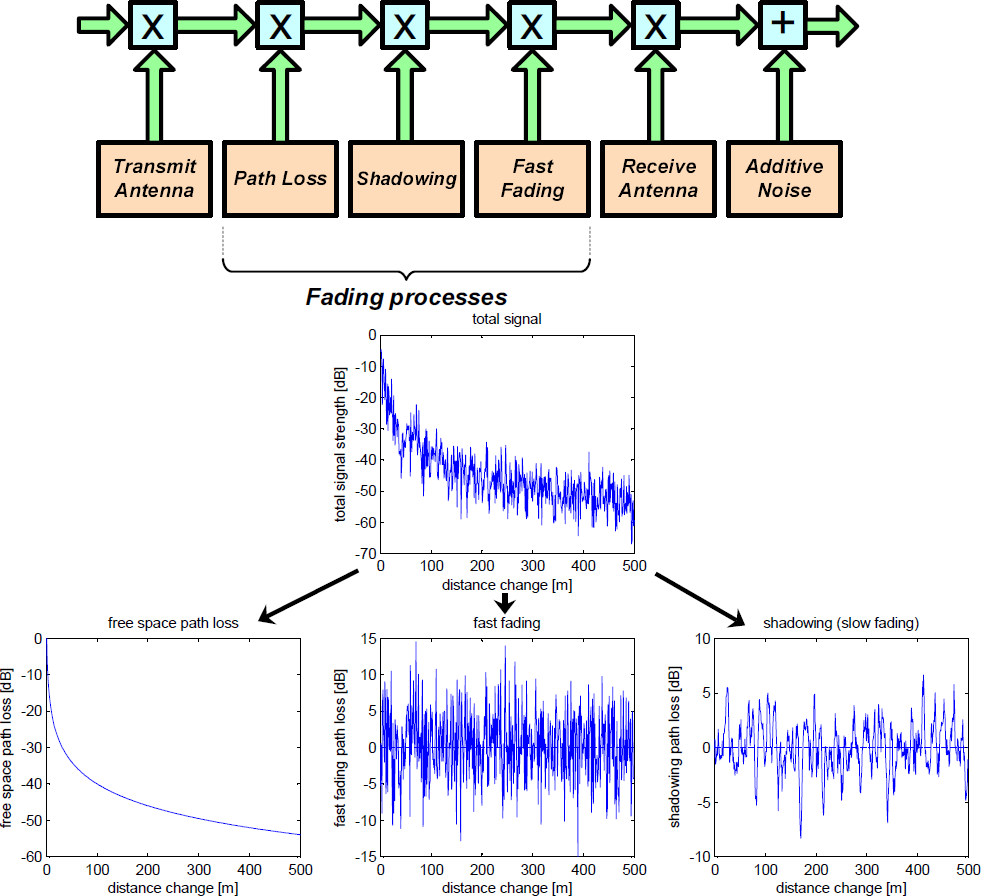
\includegraphics[width=7cm]{../MobKom2/bilder/antennas-noisetypes.png}}
& \parbox{10cm}{
    Rauschtypen:
    \begin{liste}
        \item Additives Rauschen
        \begin{liste}
            \item Thermisches, Flicker/Funkel/$\frac{1}{f}$, Shot Rauschen
            \item Atmosph�rischer Einfluss, Kosmische Strahlung, St�rungen von
            anderen el. Quellen
        \end{liste}
        \item Multiplikatives Rauschen
        \begin{liste}
            \item Richtungsabh�ngigkeit der Antennen
            \item Reflektionen
            \item Absorptionen
            \item Streuungen (Scattering)
            \item Beugung (Diffraction)
            \item Brechnung (Refraction)
        \end{liste}
    \end{liste}}
\end{tabular}
\subsection{Einf�hrung }
\begin{liste}
    \item Pfadverlust in Kabel: Linear zur Distanz; in der Luft: Logarithmisch zur Distanz
    \item Nah- \& Fernfeld: Grenze bei $R = \frac{2L^2}{\lambda}$
    \item Impedanz in der Luft: 
    $Z=\frac{|E|}{|H|}=\sqrt{\frac{\mu_0}{\varepsilon_0}}=120\pi \,\Omega= 377\,\Omega$
\end{liste}
\subsection{Rauschen}
\subsubsection{Weisses Rauschen}
\begin{center}
	\begin{minipage}{8cm}
		$S_{XX}(\omega) = \dfrac{\eta}{2} \qquad R_{XX}(\tau) = \dfrac{\eta}{2} \cdot \delta(\tau)$ \\ \\
		Beispiel: therm. Rauschen von Widerst�nden \\
		\textbf{Nimmt} in der Praxis im \textbf{Tera-Hz Bereich ab}!
  	\end{minipage}
	\begin{minipage}{10cm}
		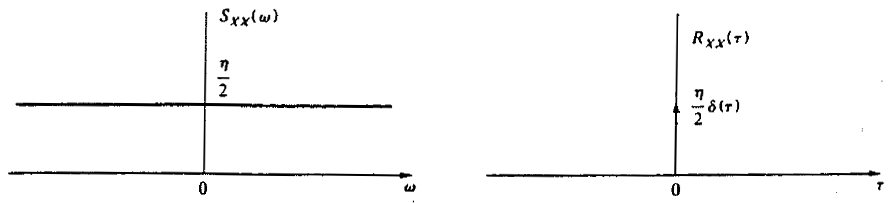
\includegraphics[width=9cm]{../NaT2/bilder/07_weisses_rauschen.png}
  	\end{minipage}
\end{center}

\subsubsection{Bandbeschr�nktes Rauschen}
\begin{center}
	\begin{minipage}{8cm}
		$S_{XX}(\omega) = \begin{cases}
                      \dfrac{\eta}{2} & |\omega| \leq \omega_B \\
                      0 & |\omega| > \omega_B
                      \end{cases} \\ \\
		R_{XX}(\tau) =  \frac{1}{2\pi} \int\limits_{-\omega_{b}}^{+\omega_{b}}
                                           \frac{\eta}{2}  \cdot e^{j\omega\tau}\; d\tau
                      = \frac{\eta\omega_{B}}{2\pi} \frac{\sin(\omega_{B}\tau)}{\omega_{B}\tau}$
  	\end{minipage}
	\begin{minipage}{10cm}
		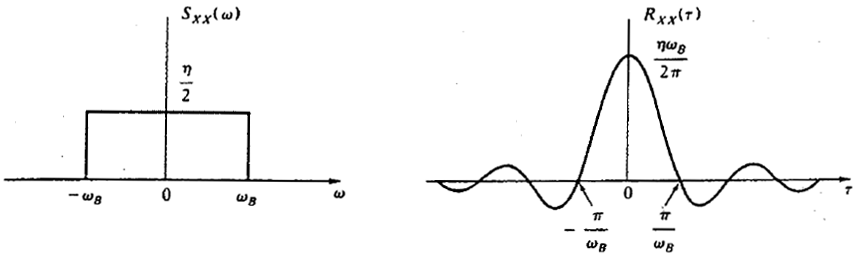
\includegraphics[width=9cm]{../NaT2/bilder/07_bandlimited_whitenoise.png}
  	\end{minipage}
\end{center}

\subsubsection{SNR}
Wegen dem Eigenrauschen $\text{N}_{\text{out,total}}$ des Verst�rkers ist das
$\text{SNR}$ am Ausgang des Verst�rkers kleiner (also schlechter) als dasjenige am Eingang. Diese Differenz ist durch die noise figure NF (in dB)
oder den noise factor $F$ (linear) gegeben.
\vspace{0.1cm}\\
$ \boxed{F = \dfrac{\text{SNR}_{\text{in}}}{\text{SNR}_{\text{out}}} =
\dfrac{\text{N}_{\text{out,total}}}{\text{N}_{\text{out,source}}}=
\dfrac{\text{N}_{\text{out,total}}}{\text{G}\cdot \text{N}_{\text{in}}}}
\qquad \Longleftrightarrow \qquad \boxed{\text{NF} = 10 \cdot \logd (F) =
\text{SNR}_{in.dB} - \text{SNR}_{out.dB} =
\text{N}_{\text{out,total,dB}}-(\text{G}_{dB}+ \text{N}_{\text{in,dB}})}$
\vspace{0.1cm}\\
$ N_{in} = k T B \qquad \text{mit } k = 1.38 \cdot
10^{-23} \qquad (k T_0)_{dB} |_{T_0 = 290K} = -174 \text{dBm/Hz} \qquad
N_{in,dB} = (k T_0)_{dB} + 10 \logd (B)$ \\
\vspace{0.1cm}
Die Bandbreite $B$ des Rauschen
$N_{in}$ ist durch das schmalbandigste Filter in einer Kaskade definiert.
\vspace{0.2cm}
Ver�nderung der SNR bzgl. Rauschen: $\qquad \text{SNR}_{out.dB} <
\text{SNR}_{in.dB} \qquad \text{SNR}_{out.dB} = \text{SNR}_{in.dB} - \text{NF}
= (S_{in.dB} - N_{in.dB}) - \text{NF}$

\begin{tabular}{ll}
\parbox{9cm}{
    \textbf{Kaskadierte Bl�cke} \\
    $$G = G_1 \cdot G_2 \cdot \cdot \cdot G_k \qquad G_{dB} = G_{1.dB} + G_{2.dB} + \cdot \cdot
    \cdot + G_{k.dB}$$
    $$F=F_1+\dfrac{F_2-1}{G_1}+ \dfrac{F_3-1}{G_1G_2}+\ldots
       + \dfrac{F_K-1}{G_1G_2\cdots G_{K-1}}$$
       $$\text{Unendliche Kaskade: }F_{\infty} = F + \dfrac{F-1}{G-1} =
       \dfrac{G \cdot F-1}{G-1}$$ F�r passive Komponenten gilt: $F =
       \frac{1}{G_{passive}}; G = G_{passive}$ }
& \parbox{9cm}{
        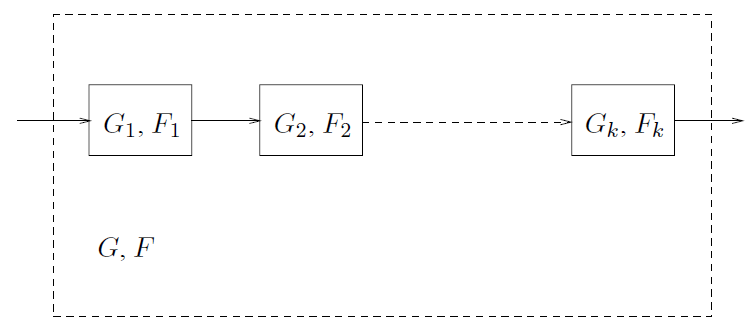
\includegraphics[width=9cm]{../MobKom1/bilder/components_amplifier_noise_cascade.png}
        }\\
\end{tabular}\\

Grunds�tzlich \textbf{dominiert} das \textbf{erste Element} einer Kaskade die noise figure NF. Ist dessen noise factor
$F_1$ klein und die Verst�rkung $G_1$ gross, so wird der gesamte noise factor $F$ klein. Dies sind
u.a. Eigenschaften von LNA-Verst�rkern.\\

\begin{tabular}{ll}
\parbox{12cm}{
    \textbf{Funkelrauschen - flicker noise} \\
    Bei tieferen Frequenzen $f$ domitiert das Funkel- oder auch 1/f-Rauschen gegen�ber dem
    thermischen Rauschen. \\ \\
    \parbox{8cm}{
    \begin{tabular}{|l|l|}\hline
    Element & corner frequency $f_c$ \\ \hline \hline
    Si-bipolar transistors & 100\,Hz to 1\,kHz \\ \hline
    Si-MOSFET              & 100\,Hz to 1\,MHz \\ \hline
    GaAs-MESFET            & 1\,MHz to 50\,MHz \\ \hline
    \end{tabular}
	}
    \parbox{3cm}{
    $F=F_0 \cdot \left(\frac{f_c}{f}+ 1\right)$
    }
 %\includegraphics[height=2.5cm]{../MobKom1/bilder/components_amplifier_noise_flicker_table.png}
    }
& \parbox{6cm}{
        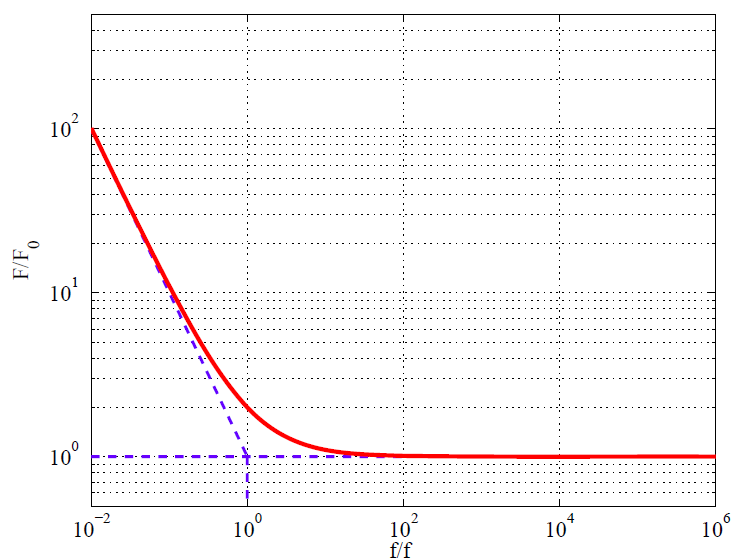
\includegraphics[height=4cm]{../MobKom1/bilder/components_amplifier_noise_flicker.png}
        }\\
\end{tabular}

\subsection{Luftlose �bertragung}
\begin{tabular}{|l|c|}
\hline
\textbf{Modell}
    & \textbf{Abbildung}\\
\hline
\hline
\parbox{10cm}{
    \textbf{Free-space propagation} \\
    \begin{minipage}{6cm}
	    \begin{liste}
	        \item Keine Reflektionen
	        \item Keine Hindernisse
	        \item Kein Multipath
	        \item Zu optimistisch/idealisiert
	    \end{liste}        
    \end{minipage}
    \begin{minipage}{3cm}
        $$ P_R= \frac{P_TG_T}{4\pi r^2} A_R $$
        $$ \frac{P_R}{P_T} = G_TG_R \left(\frac{\lambda}{4\pi r}\right)^2  $$
    \end{minipage}

    $$L=\frac{P_TG_TG_R}{P_R} = \left(\frac{4\pi r}{\lambda}\right)^2 =
    \left(\frac{4\pi rf}{c}\right)^2$$ 
    $$L\,\text{[dB]} = -147.6 + 20\log r + 20\log f$$ }
    & \parbox{3cm}{
        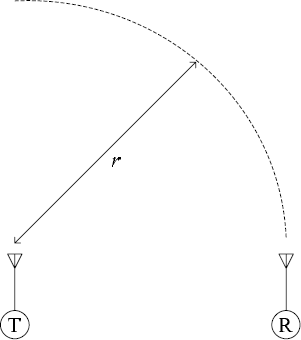
\includegraphics[width=3cm]{../MobKom2/bilder/propagation-freespace.png}
        } \\
\hline
\parbox{10cm}{
    \textbf{Open-field/Plane-earth propagation} \\
    \begin{liste}
        \item Keine Hindernisse    
        \item Einfache Reflektion am Boden (zwei Pfade)
        \item Zweiter Pfad kann konstruktiv oder destruktiv sein
    \end{liste}
    $$L= 4\frac{\pi r}{\lambda}^2
       \sin^{-2} \frac{2\pi h_bh_m}{\lambda r} \quad \text{f�r } r <
       r_x=\frac{4h_bh_m}{\lambda}$$ 
    $$L= \frac{r^4}{h_b^2h_m^2} \quad \text{f�r } r > r_x$$
    }
    & \parbox{5cm}{
        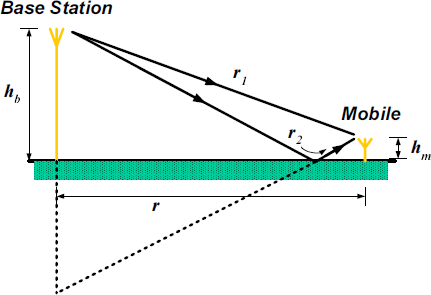
\includegraphics[width=5cm]{../MobKom2/bilder/propagation-openfield.png}
        } \\
\hline
\end{tabular}\\
\begin{tabular}{|l|c|}
\hline
\parbox{10cm}{
    \textbf{Simulation (rechts)}:\\
    $h_b=20\,$m, $h_m=1.5\,$m, $f=1\,$GHz \\
    
    \textbf{Weitere Modelle}\\
    Exponent $n$ der Entfernung $r^n$ haupts�chlich massgebend f�r Modell.
    Weitere M�glichkeiten:
    
    \begin{tabular}{|l|r|}
	\hline
	environment & path-loss exponent $n$      \\ \hline \hline
	free space                     & 2        \\ \hline
	open field (long distance)     & 4        \\ \hline
	cellular radio, urban area     & 2.7--4   \\ \hline
	shadowed urban cellular radio  & 5--6     \\ \hline
	in building, line-of-sight     & 1.6--1.8 \\ \hline
	in building, obstructed        & 4--6     \\ \hline
	\end{tabular}
    }
    & \parbox{8cm}{
    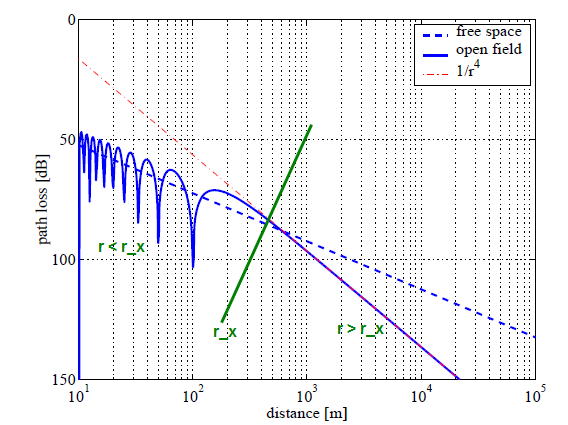
\includegraphics[width=8cm]{../MobKom2/bilder/propagation-simulation.png}
    } \\
\hline
\parbox{10cm}{
    \textbf{Okumura-Hata}:\\
    \begin{liste}
        \item Transmit frequency: f = 150...1500 MHz
        \item Height of base station antenna: $h_{BS}$ = 30...200 m
        \item Height of mobile station antenna: $h_{MS}$ = 1...10 m
        \item Distance: 1...20 km
    \end{liste}
    Path-Loss for urban enviroment:\\
    $L_{Hu}[dB] = 69.55+26.16 \logd( \frac{f}{MHz})- 13.82
    \logd(\frac{h_{BS}}{m})  - a(h_{MS}) + (44.9-6.55 \logd(\frac{h_{BS}}{m})) 
    \logd(\frac{d}{km}) $ \\
    } 
    & 
\parbox{8cm}{
  \textbf{Korrekturtur terme}:\\
    \begin{liste}
    	\item small and medium sized cities: \\
    	$a(h_{MS})=(1.1 \logd \frac{f}{MHz}- 0.7) \frac{h_{MS}}{m} - (1.56\logd 
    	(\frac{f}{MHz})-0.8)$
    	\item Metropolises:\\
    	$a(h_{MS})=\{^{(8.29 [\logd(1.54 \frac{h_{MS}}{m}) ]^2- 1.1) f\leq 200 MHz}
    	_{(3.2 [\logd(11.75 \frac{h_{MS}}{m}) ]^2- 4.97)  f\geq 400 MHz}$
    	\item sub-Urban: \\
    	$L_{Hs}[dB]=L_{Hu}-2 [\logd(\frac f{28MHz})]^2 -5.4$
    	\item rural areas:\\
    	$L_{Hr}[dB]= L_{Hu} - 4.78[\logd(\frac f{MHz})]^2 + 18.33 \logd(\frac
    	f{MHz}) - 40.94$
    \end{liste}
     } \\
\hline
\hline 
\parbox{10cm}{
    \textbf{Beugung (Diffraction)}:\\
    \begin{liste}
        \item Weitere Verluste durch Beugung
        \item Beugungsparameter: $v=h\sqrt{\dfrac{2(d_1+d_2)}{\lambda d_1d_2}}$
        \item Zus�tzlicher (zum Modell dazu) Pfadverlust: \\
        $L \approx 20\log (\sqrt 2\pi v) \approx 20\log \frac v{0.225} \quad
        v>1$
    \end{liste}
    \center{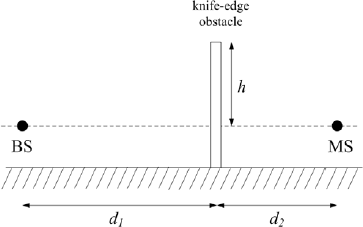
\includegraphics[width=5cm]{../MobKom2/bilder/propagation-diffraction.png}}
    }
    & \parbox{7cm}{
    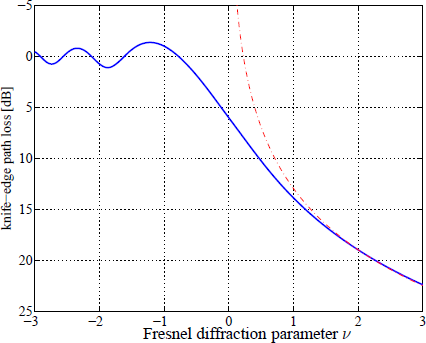
\includegraphics[width=7cm]{../MobKom2/bilder/propagation-fresnel-diffraction-parameter.png} } \\
\hline
\end{tabular}

\begin{tabular}{ll}
\parbox{11cm}{
	\subsection{Link Budget}
	\begin{liste}
	    \item Summierung aller (logarithmischen) Verluste und Gewinne vom Sender
	    zum Empf�nger
	    \item Noise power density (Rauschleistung) $N_0 = -174\text{dBm}$ (pro Hz)
	    \item Empf�nger- \& Sendergewinn ($G_T, G_R$) in DBi
	    \item Bsp: $P=N_0+10 \logd B+\text{NF}+\text{SNR}+L-G_T-G_R$
	\end{liste}

	\subsection{Shadowing (Slow Fading)}
	\begin{liste}
	    \item Tritt bei langsamen Bewegungen auf
	    \item Leichtes Entzerren, da hohe Korrelation
	    \item Normalverteilter Pfadverlust
	\end{liste}
    }
& \parbox{7cm}{
    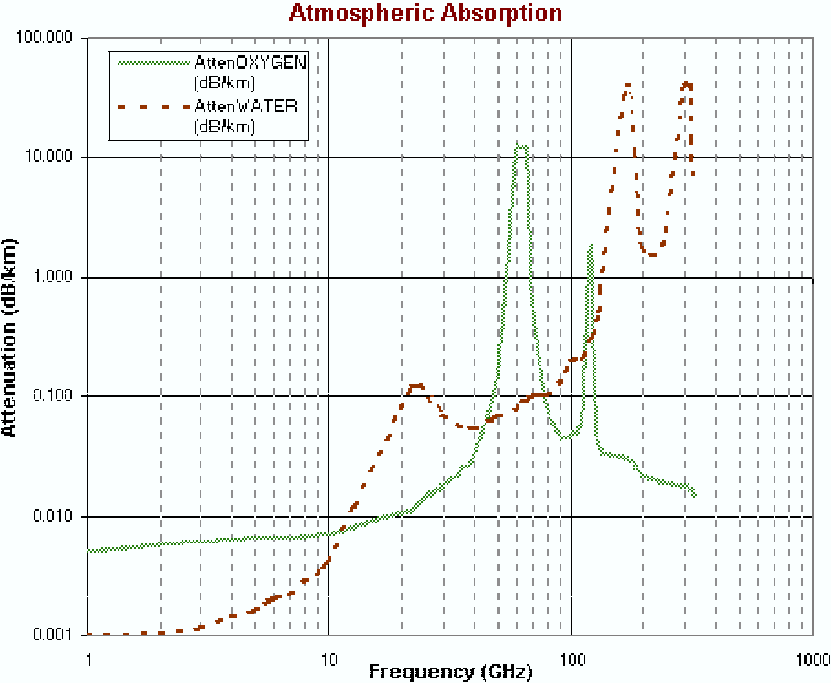
\includegraphics[width=7cm]{../MobKom2/bilder/propagation-atmospheric-absorption.png}}
\end{tabular}

\subsection{Fast Fading}
\begin{tabular}{|lll|}
\hline
\parbox{7cm}{
    \textbf{Non-line-of-sight (NLOS)} \\
    \begin{liste}
        \item Geh�rt zu flat fading (frequency non-selective)
        \item Rayleigh Verteilung $p(r) = \frac r{\sigma^2}
        e^{-\frac{r^2}{2\sigma^2}}$
    \end{liste}
    }
    & \parbox{5cm}{
        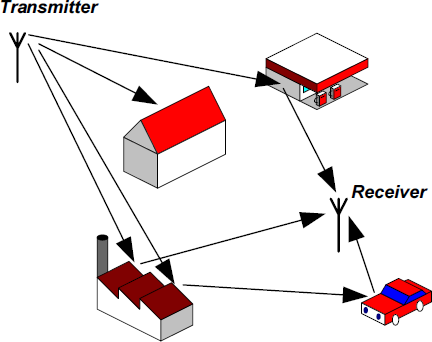
\includegraphics[width=5cm]{../MobKom2/bilder/propagation-nlos.png}
        } 
    &
    \multirow{2}{*}{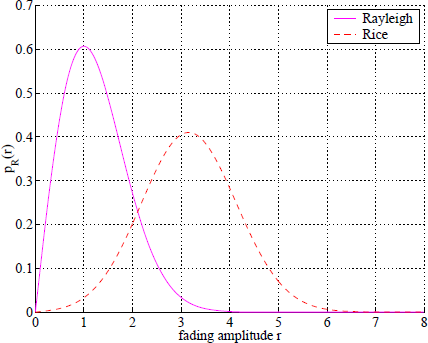
\includegraphics[width=5.5cm]{../MobKom2/bilder/propagation-fading-pdf.png}}
    \\
\parbox{7cm}{
    \textbf{Line-of-sight (LOS)} \\
    \begin{liste}
        \item Geh�rt zu flat fading (frequency non-selective)
        \item Rayleigh Verteilung $p(r) = \frac r{\sigma^2}
        e^{-\frac{r^2}{2\sigma^2}}$
    \end{liste}
    }
    & \parbox{5cm}{
        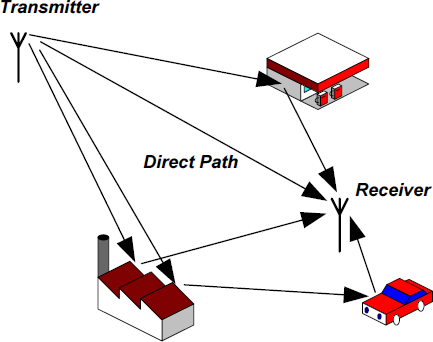
\includegraphics[width=5cm]{../MobKom2/bilder/propagation-los.png}
        } 
    & \\
\hline
\parbox{7cm}{
	    \textbf{Frequency selective fading (multipath)}
	    \begin{liste}
            \item {\em Mean delay}: $\tau_0=\frac 1{P_T}\sum\limits_k P_k
            \tau_k$
            \item {\em RMS delay spread}:\\
            $\tau_{\text{RMS}}=\sqrt{\frac{1}{P_T}}\sum\limits_k P_k
            (\tau_k-\tau_0)^2$
            \item Total power:
            $P_T=\sum\limits_k P_k$
        \end{liste}
    } 
    & \parbox{5cm}{
        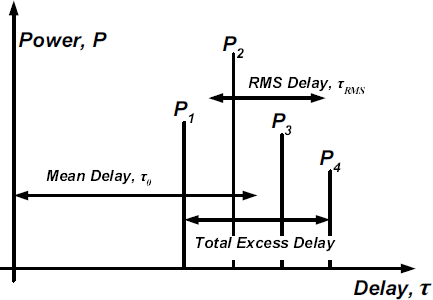
\includegraphics[width=5cm]{../MobKom2/bilder/propagation-frequency-selective-power-delay.png} 
        } 
    & \parbox{5cm}{ 
        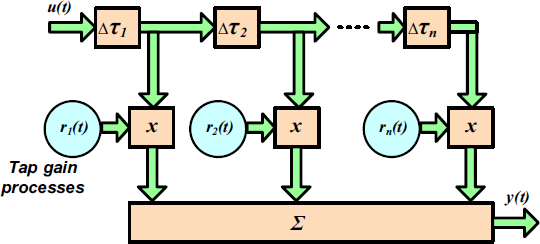
\includegraphics[width=5.5cm]{../MobKom2/bilder/propagation-frequency-selective-model.png} 
        } \\
\hline
\end{tabular}

\subsection{Beziehungen zwischen Fading Parameter}
\begin{liste}
    \item $T_c \propto  \frac 1{f_m}$ \qquad $T_c$ = Koh�renzzeit, $f_m$ =
    Dopplerverschiebung (spread)
    \item $B_c \propto \frac 1{\tau}$ \qquad $B_c$ = Koh�renzbandbreite, $\tau$
    = Zeitverbreiterung (broadeing)
    \item $B_c$, $T_c$ unabh�ngig
\end{liste}
